\chapter{Design}

The core problem to solve is finding the best way to capture updates from
either the database or filesystem and present them on the other. There were two
main alternative approaches that could be taken in order to create a system
that would solve this problem.

The first approach is the most straightforward and requires a program to be
watching the database and filesystem for changes. Once a change is detected it
would then be mirrored by applying the corresponding changes in the opposite
system. For example, if a file was created on the filesystem a record would be
created in the database.

The second approach is more complicated than the first but implements a similar
idea. Instead of creating a program which monitors the standard filesystem for
changes we create a filesystem that can be mounted on the users system and
provides live updates of any changes through a system of callbacks.

An example of operations and their corresponding action in the other system is
shown in table \ref{tbl:mappings}.

\begin{table}
	\centering
	\begin{tabular}{|l|l|}
		\hline
		\textbf{Filesystem Action} & \textbf{Database Action} \\
		\hline
		Add a file & Create a record \\
		Remove a file & Delete a record \\
		Modify a file & Change a record \\
		Rename a directory & Rename a table \\
		\hline
	\end{tabular}
	\caption{Filesystem to/from Database Mappings}
	\label{tbl:mappings}
\end{table}

\section{Polling or Filesystem?}

\subsection{Polling}

The polling system, as outlined above, would be run at regular intervals to
give the illusion that both systems were directly linked. There are numerous
challenges with this implementation with the most prominent being detecting the
changes made on each side. Triggers that will execute when changes are made or
streaming logs of all changes can be used to monitor for changes in a database.
However, not all database management systems have support for these features.

Waiting for changes in a filesystem is possible simply by scanning over the
filesystem for any modification dates that have changed since the last scan was
performed. However, this syster is very ``brute force'' and may be slow on
systems with many files. To improve upon this method we may use operating
system APIs that allow us to register for callbacks when files are changed. The
libraries to perform these tasks are \texttt{inotify} for Linux and
\texttt{fs-events} for Mac OS X.

This is a less than ideal solution for checking for updates when we may have
millions of records and therefore millions files that need checking. This
solution just does not scale well even with the operating system assistance.
Additionally, the constant polling of the filesystem is a lot of wasted work
that will deplete the battery of laptops unnecessarily and waste power on
desktop machines. Instead, we should flip the problem around and instead of
looking for the files that have been changed, we should get any file that
changes to tell us about itself.

\subsection{Filesystem}

By using a filesystem instead of an separate polling program we tighten the
feedback loop from changes to the files to the database. By doing this we avoid
the potentially expensive operations of scanning the filesystem for changes and
have direct callbacks that reference the exact file changed. This has the
additional advantage of automatically handling migrating any changes back from
the database to the filesystem just by refreshing the current view.

% TODO: Add more stuff.

\section{Scaling Issues}

There is some concern about how this system scale up to the sizes that some
databases can and will reach. This is due to some unknowns as to how
a filesystem will perform once it has millions of files in it with each file
representing a record in the database. In order to mitigate this problem (if it
does exist) the files should be nested more deeply in a tree structure in order
to reduce the number of files in a directory down to reasonable levels.

Since users rightly demand that a filesystem is responsive at all times then
a non-functional requirement should be made that the database returns all
queries as quickly as reasonably possible. There are numerous ways that this
could be achieved such as the simple caching of values outside the database in
memory all the way up to using previous usage patterns to scan across the data
on the disk in order to load it into memory before the query is ever made and
creating useful indexes automatically to help regularly slow queries. However,
it is unwise to spend unnecessary time considering solutions to problems that
may not occur.

\section{The Querying Problem}
\label{sec:queryproblem}

A database has 4 main duties when it comes to presenting the user with data:
adding, updating, deleting, and updating. Our current solution to the problem
provides a good solution to adding, updating, and deleting records but querying
the database beyond basic operations is not easy to do with the limited actions
available to the filesystem. When querying or searching a filesystem, one would
normally use commands such as \texttt{find} or \texttt{grep}. These commands
take far too long to provide the desired results when presented with this many
files. Additionally, they are also not set up to use the information that
a database can provide when querying such as having ordering defined on
records.

In order to allow the user to perform more complex queries on the database
a separate application is needed. However it is critical that still presents
the database as a filesystem. If we look at how users perform complex sequences
of operations on a filesystem: there are two different approaches depending on
the level of expertise of the user.

\subsection{Mirroring Filesystem Solutions}

If we have a task that we would like to perform such as resizing all of the
images in a folder that were taken in the last week and which have the word
``flower'' in the filename then depending on the level of expertise of the user
they will probably approach this problem in two different ways.

A technical user will could write a shell script or use multiple commands
piped together to achieve the intended effect. A command such as the following
will perform the task shown in figure \ref{fig:shell}.

\begin{figure}[ht!]
  \centering
	\begin{verbatim}
	  find . -type f -name ".jpg" |
	    grep "flower" |
	    xargs convert -resize 50%
	\end{verbatim}
  \caption{Shell Workflow}
  \label{fig:shell}
\end{figure}

Instead of performing the action in one step the user splits up the command
into 3 logical steps of find the pictures, filter the ones with flower in the
name, and finally perform the resizing. There is a flow of data through the
series of commands that are used.

A non-technical user has a number of available operations to them. The most
widely used among Macintosh users is probably a program named \emph{Automator}
which is bundled with the operating system and integrates well with it. It
allows the user to create a similar workflow to shell scripts by composing
a sequence of similar duties to the programs above. An example of an
\emph{Automator} workflow is shown in figure~\ref{fig:automator}. This workflow
performs the same task as described above.

\begin{figure}[ht!]
  \centering
  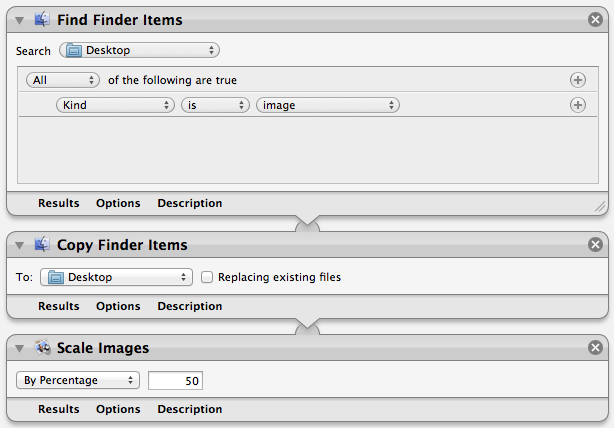
\includegraphics[width=0.9\textwidth]{images/automator}
  \caption{Automator Workflow}
  \label{fig:automator}
\end{figure}

We should be able to take this existing solution and paradigm and apply it to
the database querying problem. I believe that this will work especially well if
we make the records maintain their file-like qualities even inside the
application. In order to convert this graph of command into a database action
we are going to need to generate \ac{SQL} which will perform the desired
action. This is the next design challenge.

\subsection{Creating SQL}

The task of creating \ac{SQL} has been solved many different times when
creating \acp{ORM}. These often use Relational Algebra or something similar to
represent the compound operators before being converted to a sensible SQL
statement. Using a similar approach for this task would be sensible as it
mimics the graph structure that is described above. For example, a filter node
in the application above is equivalent to a selection wrapping everything above
it in the graph.

This intermediate relational algebra representation also has the advantage of
completing the metaphor above by replacing the more technical users requirement
of being able to drop down to a more direct interface to controlling the
database.

To this end I'm going to create an intermediate language that allows the user
to create complex \ac{SQL} queries by writing relational algebra in an
imperative style. This can then be combined with the filesystem by allowing
these files to be saved on it and having it return the results.

\subsection{Querying the Filesystem}

While more advanced users may be able to write the intermediate language
directly in order to query the database there needs to be a program to help
the majority of users to be able to use the system. The example used above
(\emph{Automator}) allows the users to create a simple flow of data through
different applications and services. We are able to see a similar pattern that
can be used to query databases by having the user create a flow that is
similar to the query graph that will be used inside the database.

The graph that the user creates can then be traversed in order to generate
the language described above.
